\section{Algorithm}%
\label{Algorithm}

% \NewCryptoEntity{\Alice}{A}
% \NewCryptoEntity{\Bob}{B}
% \NewCryptoEntity{\Carol}{C}
% % Arg, already used \mathcal{D} for the devices set
% \NewCryptoEntity{\David}{D}

\newcommand{\Alice}{\ensuremath{\mathscr{A}}}
\newcommand{\Bob}{\ensuremath{\mathscr{B}}}

\newcommand{\localoverlay}{Squad Overlay\xspace}
\newcommand{\globaloverlay}{Global Overlay\xspace}

\NewScheme{\SPOR}{SPOR}

\subsection{\(\SPOR\)}

\NewAlgorithm{\Send}{Send}
\NewAlgorithm{\Fwd}{Forward}
\NewAlgorithm{\Recv}{Receive}
\NewVariable{\rdv}{rdv}

We have the Stateless Predictive Onion Routing scheme, \SPOR, which provides 
probabilistically onion-routed message passing.
Instead of providing only one address per hop in the route (as in \eg 
Tor~\cite{Tor}), \(\SPOR\) provides several alternatives for the next hop 
depending on their probability of being online.
To do this, \(\SPOR\) provides stateless algorithms for the onion-routing.

\(\SPOR\) provides three algorithms: \(\SPOR[\Send]\) (\cref{SPORSend}), 
\(\SPOR[\Fwd]\) (\cref{SPORFwd}) and \(\SPOR[\Recv]\) (\cref{SPORRecv}).
Say Alice wants to send a message \(m\) to Bob.
Bob uses \(\SPOR[\Recv]\) to create a probabilistic onion route \(H_\rdv\) from 
a rendez-vous point to his own device swarm --- all the hops on the route are 
chosen by Bob uniformly at random.
Bob gives \(H_\rdv\) to Alice using an out-of-band channel, \eg using his phone.
Alice uses \(\SPOR[\Send]\) at some later time to send the message to Bob using 
any of her devices.
\(\SPOR[\Send]\) extends the route \(H_\rdv\) with some hops of Alice's choosing 
(uniformly randomly chosen), then starts to forward the message (using 
\(\SPOR[\Fwd]\)) through the hops on the route to Bob.
This process is illustrated in \cref{fig:file-exchange}.

\begin{figure}
  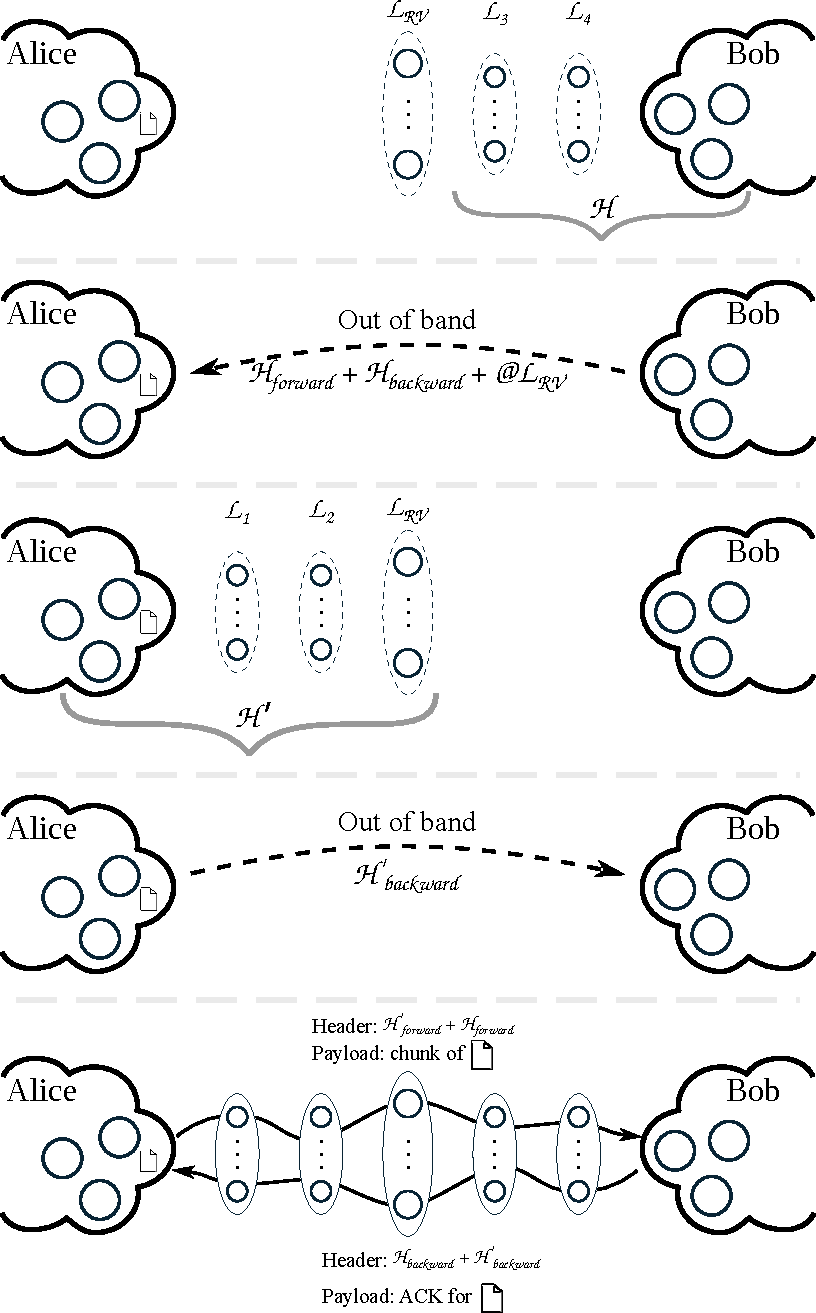
\includegraphics[width=\linewidth]{figures/file_exchange.pdf}
  \caption{\label{fig:file-exchange}%
    A schematic of Alice and Bob sending a message using \(\SPOR\).
  }
\end{figure}

\NewAlgorithm{\ExtendRoute}{ExtendRoute}
\NewAlgorithm{\GetRouteNode}{GetRouteNode}
\NewAlgorithm{\GetRandomPeer}{GetRandomPeer}

\NewAlgorithm{\Enc}{Enc}
\NewVariable{\pk}{pk}

\begin{figure}
  \begin{algorithmic}
    \Require{%
      $H$ is a header of the form \(D\concat H'\) or \(D\concat \top\), where 
      \(D\) is a set of device addresses.
      $\pk_D$ is the public key of device set $D$.
      $L$ is the length of the route,
      $\theta$ is the threshold of probability of failure.%
    }
    \Function{\ExtendRoute}{$H, L, \theta$}
      \If{$L\leq 0$}
        \State \Return $H$
      \EndIf
      \State $D\gets \GetRouteNode[\theta]$
      \State $H\gets D\concat \Enc[_{\pk_{D}}][H]$
      \State \Return $\ExtendRoute[H, L-1, \theta]$
    \EndFunction

    \Function{\GetRouteNode}{$\theta$}
      \State $D\gets \GetRandomPeer$
      \While{$\prod_{d\in D} \Pr[d \text{ offline at time } t] > \theta$}
        \State $D\gets D\cup \GetRandomPeer$
      \EndWhile
      \State \Return $D$
    \EndFunction
  \end{algorithmic}
  \caption{\label{ExtendRoute}%
    The \(\ExtendRoute\) algorithm extends a route \(H\) with \(L\) hops and 
    failure threshold of \(\theta\) for each hop in the route.
    Thus the probability of failure for the extension is \(1 - (1 - \theta)^L\).
    The function \(\GetRandomPeer\) is any random peer-sampling algorithm.
  }
\end{figure}

\NewAlgorithm{\Store}{Store}
\NewAlgorithm{\Dec}{Dec}
\NewVariable{\sk}{sk}

\begin{figure}
  \begin{algorithmic}
    \Require{%
      $D$ is the set of alternative recipient devices.
    }
    \Function{\SPOR[\Recv]}{$D$}
      \State $H_\rdv\gets \ExtendRoute[D\concat \top, L, \theta]$
      \State \Return $H_\rdv$
        \Comment{Give to sender out-of-bound.}
    \EndFunction

    \Function{\Store}{$c_m$}
      \State $m\gets \Dec[_{\sk_D}][c_m]$
      \If{$m = \bot$}
        \State \Return $\bot$
      \EndIf
      \State Store $m$ to disk.
      \State \Return $\top$
    \EndFunction
  \end{algorithmic}
  \caption{\label{SPORRecv}%
    The \(\SPOR[\Recv]\) algorithm prepares the recipient for receiving a file.
    It creates a probabilistic onion-route from a rendez-vous point to its own 
    devices and returns the route to the sender.
    The \(\Store\) algorithm is used by the local \(\SPOR[\Fwd]\) algorithm to 
    store messages intended for itself.
  }
\end{figure}

\begin{figure}
  \begin{algorithmic}
    \Require{%
      $m$ is the message to be sent,
      $\pk_D$ is the public-key of the recipient,
      $H_\rdv$ is the onion-route given by the recipient.
    }
    \Function{\SPOR[\Send]}{$m, \pk_D, H_\rdv$}
      \State $H\gets \ExtendRoute[H_\rdv, L, \theta]$
      \State $c_m\gets \Enc[_{\pk_D}][m]$
      \State $D\concat C_H\gets H_\rdv$
      \For{$d\in D$}
        \Comment{Uniformly randomly chosen}
        \If{$d\method \Fwd[C_H, c_m] \neq \bot$}
          \State \Return $\top$
        \EndIf
      \EndFor
      \State \Return $\bot$
    \EndFunction
  \end{algorithmic}
  \caption{\label{SPORSend}%
    The \(\SPOR[\Send]\) algorithm extends the route \(H_\rdv\) (using 
    \(\ExtendRoute\), \cref{ExtendRoute}) and sends the message \(m\) down the 
    extended route using the \(\SPOR[\Fwd]\) algorithm (\cref{SPORFwd}).
    The first node of \(H_\rdv\) is the rendez-vous point selected by the 
    recipient.
    \(\pk_D\) is the public key of the recipient.
  }
\end{figure}

\begin{figure}
  \begin{algorithmic}
    \Require{$\pk, \sk$ is the public--private key-pair of the node.}
    \Function{\SPOR[\Fwd]}{$C_H, c_m$}
      \State $H\gets \Dec[_\sk][C_H]$
      \If{$H = \bot$}
        \State \Return $\bot$
      \EndIf
      \State $\{d_i\}\concat C_H'\gets H$
      \If{$C_H' = \top$}
        \State \Return $\Store[c_m]$
      \EndIf
      \For{$d\in \{d_i\}$}
        \Comment{Uniformly randomly chosen}
        \If{$d\method \Fwd[C_H', c_m] \neq \bot$}
          \State \Return $\top$
        \EndIf
      \EndFor
      \State \Return $\bot$
    \EndFunction
  \end{algorithmic}
  \caption{\label{SPORFwd}%
    The \(\SPOR[\Fwd]\) algorithm forwards \(c_m\) down the route \(H\), 
    obtained by decrypting \(C_H\) with the node's associated private key.%
    The special value \(H = \top\) indicated the end of the route, thus \(c_m\) 
    is intended for the local node and \(c_m\) is instead sent to disk using 
    \(\Store\) (\cref{SPORRecv}).%
  }
\end{figure}

\subsection{Predictions and scheduling}

\commentDaniel{%
  We must cover how to do \(\Pr[d \text{ offline at time } t]\) as used above 
  (\cref{ExtendRoute}).%
}

\commentDaniel{%
  We must do the scheduling: \ie divide the file \(f\) into \(f_1, \dotsc, f_n\) 
  and how the size of \(f_i\) relates to transmission time and size of the 
  timeslot (for the validity of predictions).
  After that we just do \(\SPOR[\Send]\) on each \(f_i\).%
}


\subsection{Adrien's old stuff}

\commentDaniel{%
  Anything below this line should be updated, integrated or removed.%
}
A set of users $\mathcal{U}$ participate in the \name network.
Each user $u \in \mathcal{U}$ has a set $\mathcal{D}_u$ of devices that contribute to the system when online.
Alice and Bob use \name to exchange a file secretly: no participant will learn who sends and receives it, nor its content.

On one hand, a user's devices must exchange information among themselves to learn the user's behavior \commentAL{Can we skip files mapping, pretty please?} and map files to devices.
We call this part of the protocol the \localoverlay, and present it in 
\cref{local-overlay}. On the other hand, user's collectively upload the list of 
their connected devices and associated future predictions to a Distributed Hash 
Table (DHT): it serves as a registry of online peers (including connection 
probabilities for the next turn), and for the routing of files.
We describe this \globaloverlay in \cref{global-overlay}. File exchange between 
two users is enabled by the two previous protocols, and is covered in 
\cref{file-exchange}

\subsection{The \localoverlay}%
\label{local-overlay}

A user's devices, \(D_i\), use the \localoverlay to:
\begin{enumerate}
	\item Share information about the user's behavior.
	Devices use it to build a behavioral model and infer their future connection probability;
  \item Share files location \commentAL{Maybe \dots}
\end{enumerate}

\subsubsection{Sharing the user's behavior}% (fold)
\label{ssub:sharing_the_user_s_behavior}

Each device initially only knows when it is connected. 
To make a model of the user's behavior, they need to know the whole observation sequence $O$: which device is online at each time step.
To do so, they employ a probabilistic dissemination protocol, based on previous work from our team~\cite{luxey:hal-01704172}.
This algorithm, called \textsc{Sprinkler}, allows devices to gossip any new connection information to random peers, ensuring that all devices know the full observation sequence with a very high probability.
\textsc{Sprinkler} has shown resilient to devices churn~\cite{luxey:cascade}, and is thus perfectly suited for our purpose, where a user's devices often disconnect and reconnect. 

\commentAL{Then we \textbf{maybe} do predictions as \textbf{maybe} shown in 
  \cref{sec:user_model}.}


% subsubsection sharing_the_user_s_behavior (end)

\subsubsection{Sharing files location}% (fold)
\label{ssub:sharing_files_location}

We do stuff and things work.

% subsubsection sharing_files_location (end)

\subsection{The \globaloverlay}%
\label{global-overlay}

% All swarms participate in the Inter-Swarm Protocol to coordinate the global 
% knowledge needed by the swarms to interact.
% More specifically, the global knowledge contains:
% \begin{itemize}
%   \item A table, \(R\), of devices available for routing;
%   \item A key--value store, \(S = \{0, 1\}^\lambda\times \{0, 1\}^*\), mapping 
%     fixed-length strings of length \(\lambda\) to arbitrary-length strings.
% \end{itemize}

Every device in the system participates in a Distributed Hash Table (DHT) that is used for two purposes:
\begin{enumerate}
  \item Providing routing information to nodes during file exchange. This is 
    discussed in-depth in \cref{file-exchange};
	\item Listing online devices and their probability of being online next time step.
\end{enumerate}

Every time a device is online, it sends the following information to the DHT:
\begin{itemize}
	\item the time \commentAL{step?};
	\item its address;
	\item its public key;
	\item the probability that it will still be connected next turn \commentAL{no interest in t+2 and more.}
\end{itemize}

\commentAL{Cite DHT articles and emphasize their security guarantees.}

\subsection{The file exchange}%
\label{file-exchange}

We consider two users, Alice and Bob, such that Alice wants to send a file to Bob secretly.
They want to keep the file content secret to anybody but them; \name's users should not know who sent a file to whom; and Alice and Bob want to hide their address from one another.

In other words, \name must guarantee \emph{sender-receiver anonymity}.
To achieve this, communications go through onion routes, using rendez-vous points.
Our approach is tightly based on the Tor seminal paper~\cite{Tor}.

\subsubsection{File exchange process}% (fold)
\label{ssub:file_exchange_process}

Firstly, Alice and Bob must exchange information out-of-band: an encryption key $ek$ to cipher the file, and an ID $k$ in the DHT pointing to information on how to reach Alice.

The device that contains Alice's file \commentAL{I don't like that dependence on the file's location} creates routes to several Introductory Points (IP), chosen at random among connected peers.
Alice uploads the addresses of her IP to the DHT at the position $k$.
One of Bob's devices creates routes to several Rendez-Vous points (RV), randomly picked among peers that will be connected in the next time step.
Bob fetches the addresses of Alice's IP from the \ac{DHT}.
Then, he sends a packet containing the addresses of its chosen RV to Alice's IPs.
The IP nodes forward the packet to Alice's device. 
Alice chunks her file into pieces of a predefined size, encrypted using $ek$.

Starting from the next round, Alice will send all chunks of her file to Bob's RV, that will forward it to Bob.
Once the file is received, everybody is happy and all routes are killed.

% subsubsection file_exchange_process (end)

\subsubsection{Onion routes in face of churn}% (fold)
\label{ssub:onion_routes_in_face_of_churn}

An onion route between A and B consists of several servers (usually three) that serve as relays, say $r_1, r_2$ and $r_3$. 
The route will have a fixed order: $A \rightarrow r_1 \rightarrow r_2 \rightarrow r_3 \rightarrow B$.
Every time data travels through the onion route, it is encrypted---along with its header---with symmetric keys, such that no-one except the sender and the receiver can read its content.
A node only knows its direct predecessor (that sent the packet) and its direct successor (whose address is the only one readable by it) on the route, such that only the creator of the route (A) knows the destination (B).

Alas, when one node goes down along the way, the route has to be recreated, at least partly.
Alice will be informed of the crash by the predecessor of the failed node with a control message, using the onion route.
Then, she will have to select a new connected peer, and ask the predecessor of the failed node to re-establish the route using this new peer.
This is fine in scenarii where participating servers only fail sporadically.
But in our setup, where devices disconnection is a certainty, we need a more robust approach.

We select several relays at each point of the route: $R_i=\{r_{i,j}\}$ would be the \emph{set} of possibly disconnected devices that will take the $i^\text{th}$ position in our onion route.
In traditional onion routing, $r_1$ is the only one knowing the address of $r_2$, because it is written encrypted with its public key in the header.
Here, every device in the $R_i$ can read the set $R_{i+1}$ in the header, because the symmetric key $sk$ used to encrypt the set $R_{i+1}$ is known to every device in $R_i$.
The header indeed contains a version of $sk$ for each device $r_{i,j}$, encrypted with its own public key $pk_{r_{i,j}}$.

In the following equation, $S(sk,\texttt{message})$ means that $\texttt{message}$ is encrypted with the symmetric key $sk$, while $P(pk, \texttt{message})$ means that $\texttt{message}$ is encrypted using the public key $pk$.
Follows the content of the header in our version of the onion routing, considering that $R_i=\{r_{i,1}, r_{i,2}, r_{i,3}\}$, that $pk_{r_{i,j}}$ is $r_{i,j}$'s public key, and that $||$ means concatenation:
\[
  P(pk_{r_{i,1}}, sk) || P(pk_{r_{i,2}}, sk) || P(pk_{r_{i,3}}, sk) || S(sk, 
  R_{i+1})
\]

(I read that this is how PGP handles multiple recipients.)



% subsubsection onion_routes_in_face_of_churn (end)

% \begin{figure}[t]
% \centering
% 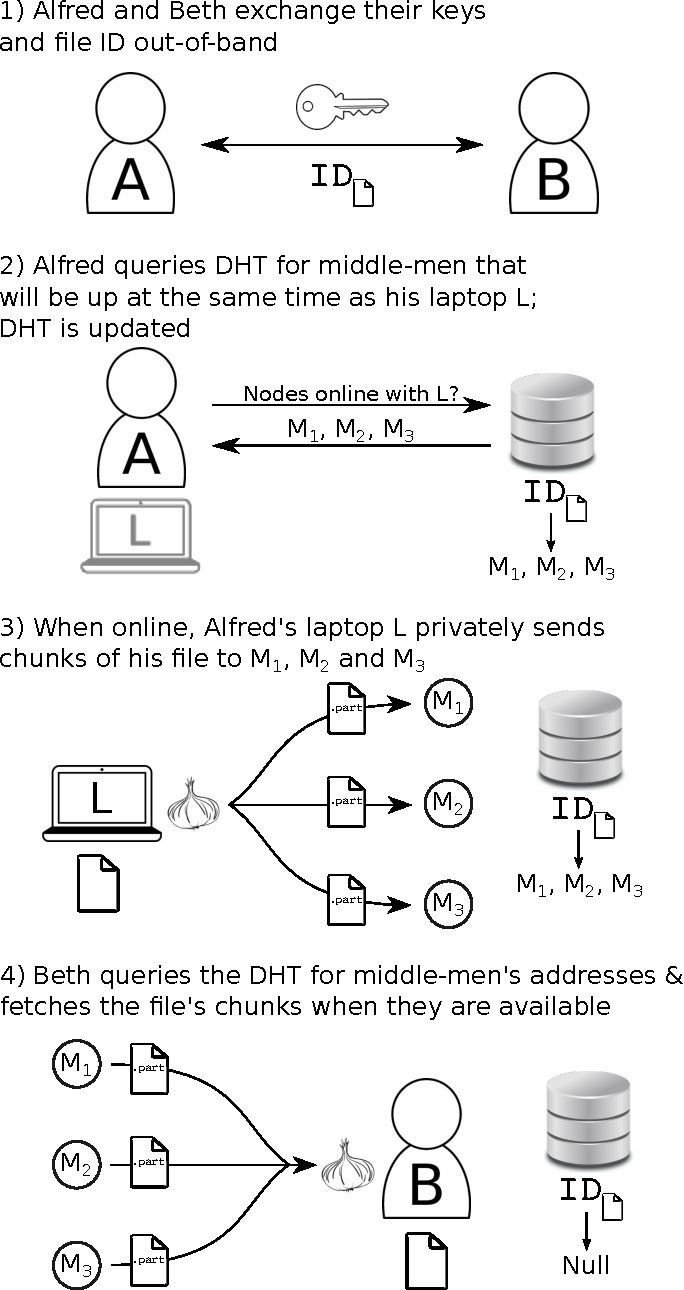
\includegraphics[width=0.8\columnwidth]{figures/schema.pdf}
% \caption{\label{fig:pipeline}Pipeline of the steps undergone by Alice when he shares a file from his laptop L with Bob.}
% \end{figure}

% \Cref{fig:pipeline} depicts the process of a file exchange from Alice to Bob.
% The file $f$ is initially located on Alice's laptop $L$, which is potentially offline for now.
% Firstly, Alice and Bob need to exchange encryption keys and the key $ID_f$ 
% referencing the file on the \ac{DHT}.
% They do so \emph{out-of-band}, that is using another channel than the one 
% presented here (\eg bluetooth, email, \etc).

% Then, Alice queries the DHT for devices that will most likely be online at the same time as his laptop $L$.
% To this end, Alice uses his knowledge on his devices connection patterns $A_i$, along with the DHT's public information on devices connections.
% Once Alice and the DHT agreed upon a set of peers $(M_1, M_2, M_3)$, their address is put in the DHT at the key $ID_f$ referencing the file of interest.

% At the third step, Alice's laptop $L$ becomes available. 
% Informed of the ongoing file exchange by Alice's Device Swarm Protocol, $L$ fetches the addresses of $M_1, M_2$ and $M_3$ on the DHT using the key $ID_f$.
% These peers will serve as middle-men: $L$ sends them redundant chunks of $f$ through an onion route (thus remaining anonymous), for Bob to fetch them later.

% In the last forth step, Bob fetches the file $f$ using any of her devices.
% To do so, she uses the key $ID_f$ to learn the addresses of $M_1, M_2$ and $M_3$.
% Then, she fetches parts of $f$ from the online middle-men through an onion route.
% Given that $L$ sent redundant chunks to the middle-men, Bob will not need every middle-man to be connected to fetch the whole file.
% Once Bob has completed the download, the key $ID_f$ is flushed on the DHT.
